\documentclass{elbioimp2}
\usepackage[utf8]{inputenc}

\usepackage[backend=biber,style=vancouver]{biblatex}
\usepackage{csquotes}
 \usepackage{qcircuit}

\title{The state of Quantum Computing in 2025}
% \shorttitle{Short version of title}
\author{Adam Prior.\affiliation{UrbanFox, Dublin, Ireland}} 
\shortauthor{A. Prior.}
% \elbioimpreceived{19 Sept 2025}  
% \elbioimppublished{19 Sept 2025}
% \elbioimpfirstpage{1}
% \elbioimpvolume{x}
% \elbioimpyear{20xx}
 
\addbibresource{bibliography.bib}

\begin{document}
\maketitle

\begin{abstract}
  This paper provides an accessible overview of the current state of quantum computing technologies
  as of September 2025. Aimed at readers with a technical background but no prior experience in quantum
  computing, it reviews foundational concepts, historical advancements, and leading hardware and software platforms. The paper
  also discusses practical challenges, potential applications, and the outlook for future developments in the field.

  \keywords{Quantum Computing; Quibits; Decoherence; robotics}
\end{abstract}

\section{Introduction}
This document is a template for \LaTeX. 
Please use the electronic version of this document as a
template when you produce your manuscript for submission to the
\emph{Nordic Machine Intelligence}. The paper size is A4 (21 × 
29.7~cm).

The introduction section of your paper should include the necessary
background information, including an adequate review of earlier
findings and the justification for conducting this study.

\section{Materials and methods}
The margins in this document are set to 2.5\,cm for the top and 1.5\,cm
for the sides and bottom. The main body of the manuscript is in two
columns separated by a 1\,cm. The line spacing is 1.1, and the
references list has 3\,pt spacing between each reference.

Body text is \emph{Computer Modern Bright} (which is quite similar to
Calibri) at 10\,pt. Level~1 headings are in bold and level~2
headings are in italic.

In the materials and methods section, please describe all necessary
details on how the study was performed. Do not
include any discussions of the work in this section. Enough
information should be given so that other researchers can reproduce
your study.


\section{Results}
All figures should be numbered consecutively with the figure legend
indented 0.5\,cm on each side. See figure~\ref{box-plot} for an example.
Figures may be in color or black and white and must be of such quality
that they produce clear and sharp printouts on an ordinary (color)
laser printer.

\subsection{What to include}
Use this section to present the results from the measurements or
studies that were described in the last section, but without going
into any discussion about the results.

\begin{figure}[htp]
  \centering
  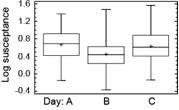
\includegraphics[width=0.7\columnwidth]{assets/test-ill}
  \caption{Box-plot showing median value (line), mean value (cross),
    middle 50\,\% (box) and smallest and largest point within 
    1.5~interquartiles from the box (whiskers) of all measurements
    on days A, B and~C.\label{box-plot}}
\end{figure}


\begin{figure}[h]
  \centering
    \scalebox{1.5}{
      \Qcircuit @C=2em @R=1em {
        & \ctrl{2} & \targ & \gate{U} & \qw \\
        & \qw & \ctrl{-1} & \qw & \qw \\
        & \targ & \ctrl{-1} & \ctrl{-2} & \qw \\
        & \qw & \ctrl{-1} & \qw & \qw
      }
  }
  \caption{Example of a simple quantum circuit. Each horizontal line represents a qubit, and the symbols show basic operations that can be performed on them.}
\end{figure}

\section{Discussion}
Now you can discuss your results. Emphasize the new and important
aspects of the study and the conclusions that follow from them. Do not
repeat in detail data or other information given in the Introduction
or the Results section. After this section there may be sections
called Conclusion and Acknowledgments. The last section is References.



\subsection{Reference style}
The journal of \emph{Nordic Machine Intelligence} uses primarily the Vancouver
style of references with numbers in square brackets in the text and a
numbered list in the Reference section.\cite{biomed-req} However, using the
Harvard reference style will also be accepted in some cases.

\subsection{Conflict of interest}
Authors state no conflict of interest. (Either keep this sentence or
describe any comflict of interest.)

\newpage
\nocite{*}
\printbibliography
\end{document}
